%% fig_rigidity.tex   (generated by make_frontier.py; do not edit by hand)
%% Rigidity of the exceptional classes on the square of a Mumford fourfold: nested Hodge loci and the nine weight blocks.
\documentclass[tikz,border=8pt]{standalone}
\usepackage{amsmath,amssymb}
\usetikzlibrary{arrows.meta,calc,decorations.pathreplacing}
%% palette.tex -- shared colour definitions for the figures
\definecolor{PInk}{RGB}{26,32,44}
\definecolor{PBlue}{RGB}{37,82,139}
\definecolor{PTeal}{RGB}{23,127,125}
\definecolor{POchre}{RGB}{193,138,44}
\definecolor{PClay}{RGB}{178,74,58}
\definecolor{PSlate}{RGB}{108,122,137}
\definecolor{PViolet}{RGB}{110,86,150}
\definecolor{WBlue}{RGB}{223,234,246}
\definecolor{WTeal}{RGB}{220,238,236}
\definecolor{WOchre}{RGB}{250,240,218}
\definecolor{WClay}{RGB}{247,229,224}
\definecolor{WSlate}{RGB}{238,241,244}
\definecolor{PMag}{RGB}{158,58,110}
\definecolor{PGrass}{RGB}{62,124,66}
\definecolor{PAmber}{RGB}{214,112,38}
\definecolor{PIndigo}{RGB}{58,64,140}
\definecolor{PRule}{RGB}{176,186,197}

%% shared macros so the standalone figures match the paper
\providecommand{\QQ}{\mathbb{Q}}
\providecommand{\ZZ}{\mathbb{Z}}
\providecommand{\RR}{\mathbb{R}}
\providecommand{\CC}{\mathbb{C}}
\providecommand{\PP}{\mathbb{P}}
\providecommand{\Kx}{K^{\times}}
\providecommand{\HW}{W}
\providecommand{\Nm}{\mathrm{N}}
\providecommand{\Hdg}{\mathrm{Hdg}}
\providecommand{\NS}{\mathrm{NS}}
\providecommand{\cA}{\mathcal{A}}
\providecommand{\cD}{\mathcal{D}}
\providecommand{\cF}{\mathcal{F}}
\providecommand{\cP}{\mathcal{P}}
\providecommand{\cO}{\mathcal{O}}
\providecommand{\cQ}{\mathcal{Q}}
\providecommand{\bbar}[1]{\overline{#1}}
\providecommand{\ch}{\operatorname{ch}}
\providecommand{\End}{\mathrm{End}}

\newcommand{\hcimp}{\,\textcolor{PIndigo}{\tiny$\Leftarrow\mathbf{HC}$}}
\begin{document}
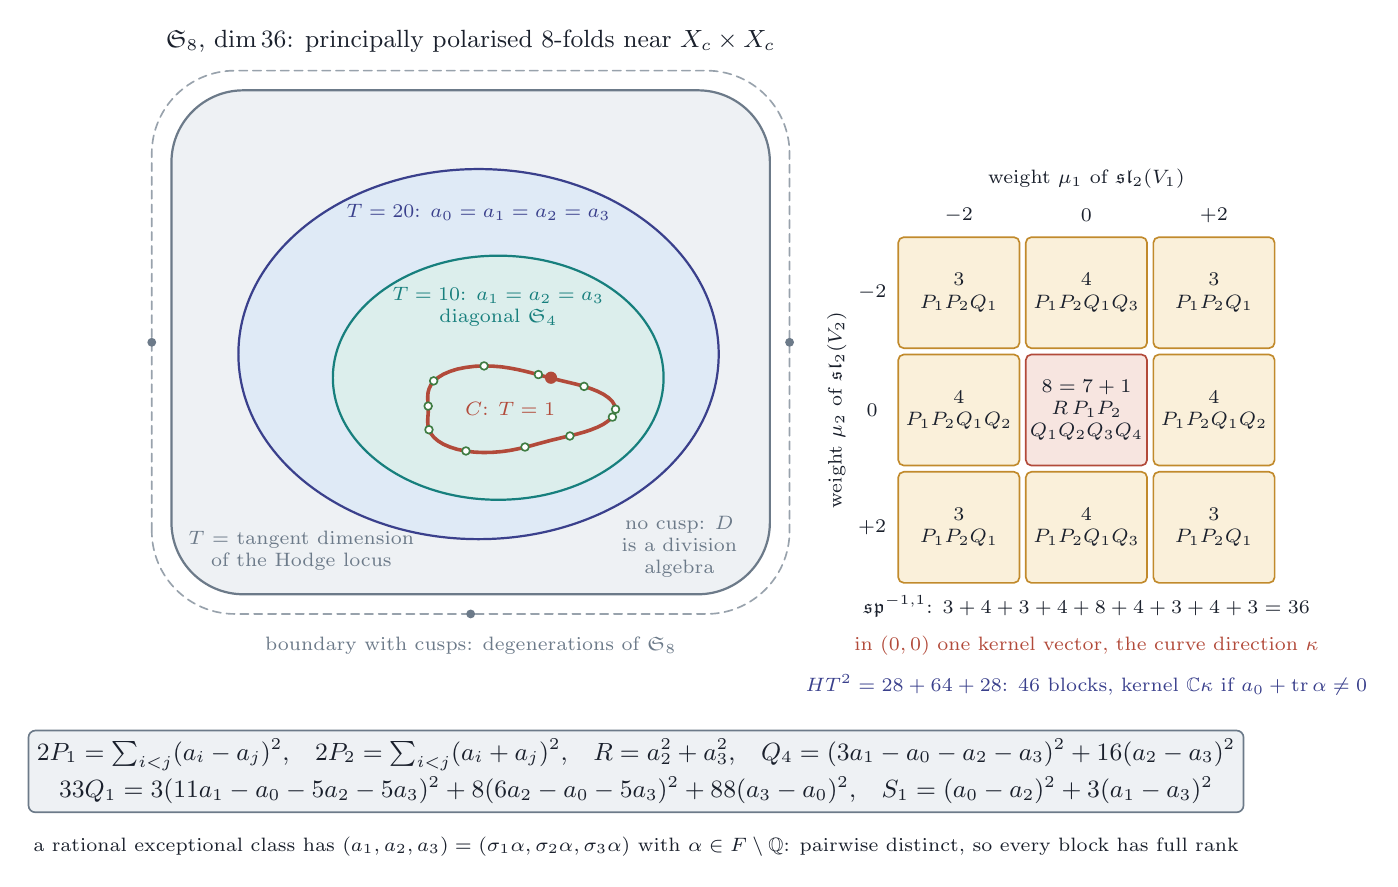
\begin{tikzpicture}[x=1cm,y=1cm,line join=round,line cap=round,
  font=\small,text=PInk]
  \draw[PSlate,fill=WSlate,line width=0.8pt,rounded corners=26pt] (-0.20,-0.30) rectangle (7.40,6.10);
  \draw[PSlate!70,line width=0.6pt,dash pattern=on 3pt off 2pt,rounded corners=30pt] (-0.45,-0.55) rectangle (7.65,6.35);
  \fill[PSlate] (-0.45,2.90) circle (1.6pt);
  \fill[PSlate] (7.65,2.90) circle (1.6pt);
  \fill[PSlate] (3.60,-0.55) circle (1.6pt);
  \node[text=PInk,inner sep=1pt,align=center,font=\small] at (3.60,6.72) {$\mathfrak{S}_{8}$, $\dim 36$: principally polarised $8$-folds near $X_{c}\times X_{c}$};
  \node[text=PSlate,inner sep=1pt,align=center,font=\scriptsize] at (3.60,-0.95) {boundary with cusps: degenerations of $\mathfrak{S}_{8}$};
  \draw[PIndigo,fill=WBlue,line width=0.80pt] (3.70,2.75) ellipse (3.05 and 2.35);
  \draw[PTeal,fill=WTeal,line width=0.80pt] (3.95,2.45) ellipse (2.10 and 1.55);
  \node[text=PIndigo,inner sep=1pt,align=center,font=\scriptsize] at (3.70,4.55) {$T=20$: $a_{0}=a_{1}=a_{2}=a_{3}$};
  \node[text=PTeal,inner sep=1pt,align=center,font=\scriptsize] at (3.95,3.35) {$T=10$: $a_{1}=a_{2}=a_{3}$\\diagonal $\mathfrak{S}_{4}$};
  \draw[PClay,line width=1.3pt] (5.438,2.050) -- (5.427,2.101) -- (5.397,2.151) -- (5.349,2.197) -- (5.286,2.240) -- (5.211,2.278) -- (5.128,2.311) -- (5.041,2.340) -- (4.952,2.365) -- (4.865,2.386) -- (4.780,2.406) -- (4.698,2.426) -- (4.619,2.445) -- (4.541,2.466) -- (4.462,2.487) -- (4.380,2.510) -- (4.293,2.532) -- (4.200,2.553) -- (4.100,2.572) -- (3.993,2.588) -- (3.881,2.597) -- (3.765,2.600) -- (3.649,2.595) -- (3.537,2.581) -- (3.431,2.560) -- (3.336,2.530) -- (3.253,2.494) -- (3.185,2.452) -- (3.133,2.407) -- (3.095,2.359) -- (3.072,2.311) -- (3.059,2.264) -- (3.055,2.217) -- (3.055,2.173) -- (3.058,2.131) -- (3.061,2.090) -- (3.062,2.050) -- (3.061,2.010) -- (3.058,1.969) -- (3.055,1.927) -- (3.055,1.883) -- (3.059,1.836) -- (3.072,1.789) -- (3.095,1.741) -- (3.133,1.693) -- (3.185,1.648) -- (3.253,1.606) -- (3.336,1.570) -- (3.431,1.540) -- (3.537,1.519) -- (3.649,1.505) -- (3.765,1.500) -- (3.881,1.503) -- (3.993,1.512) -- (4.100,1.527) -- (4.200,1.547) -- (4.293,1.568) -- (4.380,1.590) -- (4.462,1.613) -- (4.541,1.634) -- (4.619,1.655) -- (4.698,1.674) -- (4.780,1.694) -- (4.865,1.714) -- (4.952,1.735) -- (5.041,1.760) -- (5.128,1.789) -- (5.211,1.822) -- (5.286,1.860) -- (5.349,1.903) -- (5.397,1.949) -- (5.427,1.999) -- cycle;
  \draw[PGrass,fill=white,line width=0.6pt] (5.44,2.05) circle (1.4pt);
  \draw[PGrass,fill=white,line width=0.6pt] (5.04,2.34) circle (1.4pt);
  \draw[PGrass,fill=white,line width=0.6pt] (4.46,2.49) circle (1.4pt);
  \draw[PGrass,fill=white,line width=0.6pt] (3.77,2.60) circle (1.4pt);
  \draw[PGrass,fill=white,line width=0.6pt] (3.13,2.41) circle (1.4pt);
  \draw[PGrass,fill=white,line width=0.6pt] (3.06,2.09) circle (1.4pt);
  \draw[PGrass,fill=white,line width=0.6pt] (3.07,1.79) circle (1.4pt);
  \draw[PGrass,fill=white,line width=0.6pt] (3.54,1.52) circle (1.4pt);
  \draw[PGrass,fill=white,line width=0.6pt] (4.29,1.57) circle (1.4pt);
  \draw[PGrass,fill=white,line width=0.6pt] (4.86,1.71) circle (1.4pt);
  \draw[PGrass,fill=white,line width=0.6pt] (5.40,1.95) circle (1.4pt);
  \fill[PClay] (4.62,2.45) circle (2.2pt);
  \node[text=PClay,inner sep=1pt,align=center,font=\scriptsize] at (4.10,2.05) {$C$: $T=1$};
  \node[text=PSlate,inner sep=1pt,align=center,font=\scriptsize] at (1.45,0.25) {$T$ = tangent dimension\\of the Hodge locus};
  \node[text=PSlate,inner sep=1pt,align=center,font=\scriptsize] at (6.25,0.30) {no cusp: $D$\\is a division\\algebra};
  \node[draw=POchre,fill=WOchre,rounded corners=2pt,line width=0.6pt,minimum width=1.54cm,minimum height=1.41cm,inner sep=1pt,align=center,font=\scriptsize] at (9.80,3.53) {$3$\\$P_{1}P_{2}Q_{1}$};
  \node[draw=POchre,fill=WOchre,rounded corners=2pt,line width=0.6pt,minimum width=1.54cm,minimum height=1.41cm,inner sep=1pt,align=center,font=\scriptsize] at (9.80,2.04) {$4$\\$P_{1}P_{2}Q_{1}Q_{2}$};
  \node[draw=POchre,fill=WOchre,rounded corners=2pt,line width=0.6pt,minimum width=1.54cm,minimum height=1.41cm,inner sep=1pt,align=center,font=\scriptsize] at (9.80,0.55) {$3$\\$P_{1}P_{2}Q_{1}$};
  \node[draw=POchre,fill=WOchre,rounded corners=2pt,line width=0.6pt,minimum width=1.54cm,minimum height=1.41cm,inner sep=1pt,align=center,font=\scriptsize] at (11.42,3.53) {$4$\\$P_{1}P_{2}Q_{1}Q_{3}$};
  \node[draw=PClay,fill=WClay,rounded corners=2pt,line width=0.6pt,minimum width=1.54cm,minimum height=1.41cm,inner sep=1pt,align=center,font=\scriptsize] at (11.42,2.04) {$8=7+1$\\$R\,P_{1}P_{2}$\\$Q_{1}Q_{2}Q_{3}Q_{4}$};
  \node[draw=POchre,fill=WOchre,rounded corners=2pt,line width=0.6pt,minimum width=1.54cm,minimum height=1.41cm,inner sep=1pt,align=center,font=\scriptsize] at (11.42,0.55) {$4$\\$P_{1}P_{2}Q_{1}Q_{3}$};
  \node[draw=POchre,fill=WOchre,rounded corners=2pt,line width=0.6pt,minimum width=1.54cm,minimum height=1.41cm,inner sep=1pt,align=center,font=\scriptsize] at (13.04,3.53) {$3$\\$P_{1}P_{2}Q_{1}$};
  \node[draw=POchre,fill=WOchre,rounded corners=2pt,line width=0.6pt,minimum width=1.54cm,minimum height=1.41cm,inner sep=1pt,align=center,font=\scriptsize] at (13.04,2.04) {$4$\\$P_{1}P_{2}Q_{1}Q_{2}$};
  \node[draw=POchre,fill=WOchre,rounded corners=2pt,line width=0.6pt,minimum width=1.54cm,minimum height=1.41cm,inner sep=1pt,align=center,font=\scriptsize] at (13.04,0.55) {$3$\\$P_{1}P_{2}Q_{1}$};
  \node[text=PInk,inner sep=1pt,align=center,font=\scriptsize] at (9.80,4.51) {$-2$};
  \node[text=PInk,inner sep=1pt,align=center,font=\scriptsize] at (8.70,3.53) {$-2$};
  \node[text=PInk,inner sep=1pt,align=center,font=\scriptsize] at (11.42,4.51) {$0$};
  \node[text=PInk,inner sep=1pt,align=center,font=\scriptsize] at (8.70,2.04) {$0$};
  \node[text=PInk,inner sep=1pt,align=center,font=\scriptsize] at (13.04,4.51) {$+2$};
  \node[text=PInk,inner sep=1pt,align=center,font=\scriptsize] at (8.70,0.55) {$+2$};
  \node[text=PInk,inner sep=1pt,align=center,font=\scriptsize] at (11.42,4.98) {weight $\mu_{1}$ of $\mathfrak{sl}_{2}(V_{1})$};
  \node[text=PInk,inner sep=1pt,align=center,font=\scriptsize,rotate=90] at (8.25,2.04) {weight $\mu_{2}$ of $\mathfrak{sl}_{2}(V_{2})$};
  \node[text=PInk,inner sep=1pt,align=center,font=\scriptsize] at (11.42,-0.45) {$\mathfrak{sp}^{-1,1}$: $3+4+3+4+8+4+3+4+3=36$};
  \node[text=PClay,inner sep=1pt,align=center,font=\scriptsize] at (11.42,-0.95) {in $(0,0)$ one kernel vector, the curve direction $\kappa$};
  \node[text=PIndigo,inner sep=1pt,align=center,font=\scriptsize] at (11.42,-1.45) {$HT^{2}=28+64+28$: $46$ blocks, kernel $\CC\kappa$ if $a_{0}+\mathrm{tr}\,\alpha\ne0$};
  \node[draw=PSlate,fill=WSlate,rounded corners=2.5pt,inner sep=3pt,line width=0.60pt,align=center] at (5.70,-2.55) {$2P_{1}=\sum_{i<j}(a_{i}-a_{j})^{2}$,\quad $2P_{2}=\sum_{i<j}(a_{i}+a_{j})^{2}$,\quad $R=a_{2}^{2}+a_{3}^{2}$,\quad $Q_{4}=(3a_{1}-a_{0}-a_{2}-a_{3})^{2}+16(a_{2}-a_{3})^{2}$\\[1pt]$33Q_{1}=3(11a_{1}-a_{0}-5a_{2}-5a_{3})^{2}+8(6a_{2}-a_{0}-5a_{3})^{2}+88(a_{3}-a_{0})^{2}$,\quad $S_{1}=(a_{0}-a_{2})^{2}+3(a_{1}-a_{3})^{2}$};
  \node[text=PInk,inner sep=1pt,align=center,font=\scriptsize] at (5.70,-3.50) {a rational exceptional class has $(a_{1},a_{2},a_{3})=(\sigma_{1}\alpha,\sigma_{2}\alpha,\sigma_{3}\alpha)$ with $\alpha\in F\setminus\QQ$: pairwise distinct, so every block has full rank};
\end{tikzpicture}
\end{document}
